%% ========================================================================
%%							NNLS
%% ========================================================================


\chapter{Neural Networks (NN)}
\label{cha:NN}

In the last chapter of this thesis, a mathematical concept is discussed that has attracted much attention in the recent past, namely neural networks. The area of artificial intelligence (AI) in which neural networks are embedded has been the subject of an intense media hype in recent years. In 2016, for example, a computer program developed by the British company Google DeepMind succeeded for the first time in defeating Lee Sedol of South Korea, considered to be the strongest Go player in the world \cite{wiki_01}. This victory of a machine against a human being is considered to be a milestone in the field of artificial intelligence \cite{LA_Times}. Further successes were also achieved in the area of real-time games at the beginning of 2019. For the first time DeepMind's program called AlphaStar was able to defeat the world's best players in StarCraft which is considered to be one of the most challenging real-time strategy games \cite{AlphaStar}. Also Gartner, a global research and advisory firm, which publishes the well-known but definitely criticisable hype cycle representations considers AI as one of the most important technologies of recent years. In the hype cyle for emerging technologies from 2017 there are 4 out of the 32 listed technologies that can be attributed to the field of AI, such as Deep Learning or Machine Learning \cite{Gartner2017}. Also in the following years 2018 and 2019 technologies that clearly belong to the AI sector were mentioned in the hype cycle 5 and 6 times respectively \cite{Gartner2018}, \cite{Gartner2019}. This trend towards new methods based on neruonal networks can also be seen in other places, such as Kaggle. With more than one million registered users, Kaggle is one of the world's largest platforms for data science competitions and attracts teams from all over the world with prize money in the millions \cite{Kaggle}. It can be observed that, besides gradient boosting, one of the most important concepts with which to win Kaggle competitions is the concept of neural networks in various forms.   

It is therefore clear to see that on the one hand the technology behind AI has enormous potential to solve problems that have so far been assumed to be solved only by humans. On the other hand, it can be assumed that this trend is not just a short-lived phenomenon, but a continuous process leading to business solutions which are based on AI-systems. Therefore, it is even more important to understand the underlying concepts of these technologies and to discuss their applicability in the insurance industry. Whether in the end a completely automated grouping algorithm based on neural networks is possible at all or can be implemented with the available resources remains open. However, the aim of this section is to provide an overview of the basic concepts and to present case studies with insurance cashflows. Since various terms and buzzwords related to artificial intelligence are often used differently in media reports, it is useful to classify some of the most often used terms in order to show their relationship and provide a general framework which is based on \cite{Allaire2018}. 

\begin{figure}
	\centering
	\includegraphics[width=0.5\textwidth]{figures/chapter_NN/framework}
	\caption{Relation of Artificial Intelligence, Machine Learning, and Deep Learning.}
	\label{fig:framework}
\end{figure}

\begin{itemize}
	\item Artificial Intelligence: Artificial Intelligence is a branch of computer science that deals with the programming of intelligent computer systems. Due to a missing definition of the term intelligence the question which types of computer programs are included is not clearly definable. In addition to machine learning and deep learning, there are many other approaches that do not include any kind of learning but are also part of AI. 
	\item Machine Learning: Machine learning arises from this question if it is possible to design a program in such a way that it can learn how to perform a specific task automatically. Given a set of input data and the corresponding results the task is to derive rules. These rules are therefore the output of the machine learning algorithm and can then be used to derive the results for new input data. What all these methods have in common is the fact that they actually try to identify statistical patterns in the data. Thus the aim is to find a meaningful representation of the given data by projections, translations, rotations, nonlinear transformations or any other method and to apply it then to new input data. 	 
	\item Deep Learning: Deep learning, as a sub field of machine learning, focuses on the progressive learning of several levels of abstraction which are increasingly meaningful representations of the data. One can think of the method as a multistage information distillation process where in every single process step a more meaningful representation of the data is obtained. The term deep in deep learning is a reference to the multiple layers which store the abstract representations of the input data in such an algorithm. The number of layers that contribute to a meaningful representation of the data is called depth. Although there is a considerable amount of learning involved, models with several hundred layers are quite common, depending on the type of problem at hand. The concept of the neural network is a reference to the field of neurobiology and the neurons that are connected in different ways in the human brain. Although neuronal networks are not models of the human brain, it is surprising what amazing results can be achieved with such a simple idea and a sufficiently large amount of data.
\end{itemize}
After a brief classification of the terms, the next section describes the basic structure and functionality of neural networks.

\section{Fundamentals of Neural Networks}

In the previous section the functionality of neuronal networks was already described in a rather abstract way as a multi-stage information distillation process. After this high level explanation, the focus is now on pointing out which individual components make up a simple neural network and how they interact. Figure (\ref{fig:NN_overview}) shows a simplified representation of the individual components required to build one of the most basic neural networks possible. Starting point for explaining the learning process of a neural network is a data set consisting of both the input and the associated output data. If the cash flows of insurance policies are to be simulated, the individual policy parameters can be used as input data and the associated cash flows as output data. These two exogenous quantities are then processed in several steps.

\begin{figure}
	\centering
	\includegraphics[width=0.65\textwidth]{figures/chapter_NN/NN_overview}
	\caption{Simplified representation of a neural network from \cite{Allaire2018}}
	\label{fig:NN_overview}
\end{figure}

\begin{enumerate}[label=Step \arabic*:]
	\item The process is initiated by providing the input data \texttt{Input X} in a suitably format to the first layer. 	
	\item This first layer then performs a data transformation based on some weights associated with that specific layer. In the first cycle those weights are randomly initialized.
	\item The transformed output from the first layer is then passed to the next layer and serves as its input. This layer also performs a data transformation based on weights which are again initialized randomly for the first cycle.
	\item After the data has passed through the last data transformation layer of the model the transformed output values are used as \texttt{Predictions Y'}.
	\item A predefined function, called the \texttt{Loss function}, measures the quality of the network’s output by comparing the \texttt{Predictions Y'} and the \texttt{True targets Y}. The result is the \texttt{loss score}, which is used as a feedback signal to adjust the \texttt{weights} associated with the layers.
	\item The task of the \texttt{Optimizer} is to take the \texttt{loss score} as an input and update the \texttt{weights} in such a way that the \texttt{loss score} is lowered.
\end{enumerate}

\begin{remark}
	The choice of the correct loss function is of great importance. If the loss function does not correctly reflect an improvement of the model, the neural net will inevitably drift in the wrong direction.
\end{remark}
\begin{remark}
	As already explained in the previous chapters, in the specific case of cash flow matching the sum of the squared residuals would be suitable as a loss score.
\end{remark}

The above steps describe a single learning cycle for a neural network. Of course, passing the input data through the net once is not sufficient to find combinations of weights that would lead to good prediction results at all. So what learning means, is to find a set of values for all weights such that the input is mapped correctly to the output for as many different input combinations as possible. This learning is achieved by grouping the input data into so-called batches and repeatedly passing those batches through the network. Associated with a batch is the batch size which defines the number of training samples sent through the neural network before the weights are adjusted by the optimizer.  
\begin{remark}
	Three different batch size approaches can be used to learn the weights in a network.
	\begin{itemize}
		\item Batch Gradient Descent: Batch size is equal to the size of the training samples.
		\item Stochastic Gradient Descent: Batch size is equal to one.
		\item Mini-Batch Gradient Descent: Batch size is bigger than one but less than the size of the training samples.
	\end{itemize} 
\end{remark}

Depending on the design of the network there can be millions of weights that need to be learned. Adjusting those millions of weights based on the feedback signal is by far the most computing intensive part of training a network. Due to the fact that the learning process is based on a large number of similar matrix operations it is possible to use highly parallelized algorithms. The availability of relatively affordable hardware that can efficiently handle such parallelizable tasks is besides the existence of large amount of data another  major reason why neural networks took off in recent years.  

\begin{remark}
	 Compared to a pure CPU system, graphics cards with their massively parallel architecture are predestined for handling such training tasks and can therefore massively reduce the time needed to train a network.
\end{remark}

After providing an brief overview of all components used in a neural network and presenting the idea of how a network learns, the next section focuses on the internals of a single layer.

\subsection{Single neuron}

The so called neurons form the basis of every neural network and are the elements which carry out the data transformations. Each layer of a neural network consists of one or more neurons which are connected differently depending on the structure of the underlying network. The task of a neuron is to take a predefined number of input values and map them to an one dimensional output. Figure (\ref{fig:simple_neuron}) shows a single neuron with all its associated components needed to perform the data transformation given by:

\begin{figure}
	\centering
	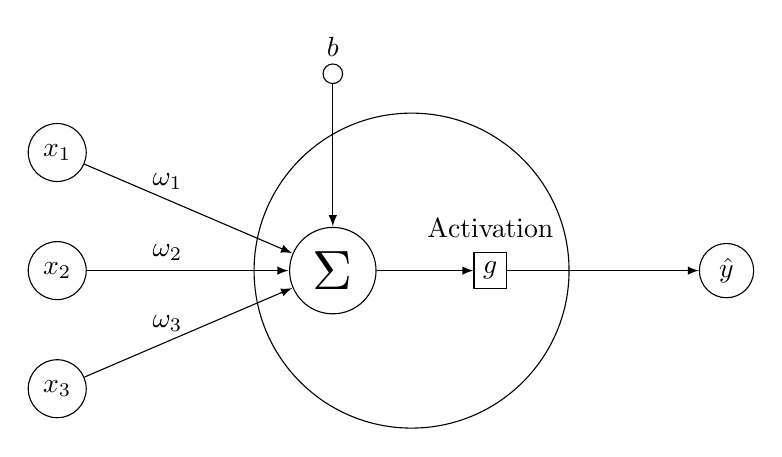
\begin{tikzpicture}[>=latex]
	\path
	(0,0)     node[circle,draw,scale=2,inner sep=2pt] (S) {$\Sigma$}
	+(90:2.5) node[circle,draw,inner sep=2.5pt] (b) {}
	node[above=1mm] {$b$}
	+(-3.5,1.5)  	node[circle, draw=black]  	(x1) 	{$x_1$}
	+(-3.5,0)    	node[circle, draw=black]  	(x2) 	{$x_2$}
	+(-3.5,-1.5) 	node[circle, draw=black]  	(x3) 	{$x_3$}
	(2,0)    		node[draw] 					(g) 	{$g$} node[above=3mm]{Activation}
	+(0:3)  		node[circle, draw=black]  	(y1) 	{$\hat{y}$};
	\draw[->] (S)--(g);
	\draw[->] (b)--(S);
	\draw[->] (g)--(y1);
	\draw[->] (x1)--(S) node[pos=.4,above]{$\omega_{1}$};
	\draw[->] (x2)--(S) node[pos=.4,above]{$\omega_{2}$};
	\draw[->] (x3)--(S) node[pos=.4,above]{$\omega_{3}$};
	\draw[black] (1,0) circle(2);
	\end{tikzpicture}

\caption{Components of a single neuron.}
\label{fig:simple_neuron}
\end{figure}

\begin{equation} \label{eq:simple_neuron}
\begin{split}
	\hat{y}		& = g\bigg( \sum_{i=1}^{3} \omega_i x_i + b \bigg) \\
				& = g(w^\top x + b) \\
				& = g(z)
\end{split}
\end{equation}
In the example shown in figure (\ref{fig:simple_neuron}) the neuron takes the three input values $x_1, x_2 \text{ and } x_3$ and transforms them in several steps into the output value $\hat{y}$. In the first step, a weighted sum is formed from the input values and the corresponding weights $w_1, w_2 \text{ and } w_3$. A bias $b$ is then added to this weighted sum and the intermediate result is called $z$. This intermediate result is then the input for the activation function $g$. Applying the activation function to $z$ gives the final output value of the neuron. The purpose of the activation function can be seen as a gate. Since both, the values of the inputs and the values of the weights are unrestricted, the value of $z$ can be in the interval (-$\infty$, $+\infty$). A natural way of determining whether the next neuron should be activated or not is to apply a transformation to $z$, which is done by an activation function. For this reason neural networks use non-linear activation functions. Those activation functions can limit the value range and also enable the network to learn complex data structures. Some of the most commonly used activation functions in neural networks are shown in figure (\ref{fig:activation_func}): 

\begin{figure}
	\centering
	\includegraphics[width=0.75\textwidth]{figures/chapter_NN/activation_functions}
	\caption{Commonly used activation functions for neural networks.}
	\label{fig:activation_func}
\end{figure}


\begin{itemize}
	\item Sigmoid function: 
		\begin{equation}
		\begin{split}
			g: \R 	& \mapsto (0,1) \\
			g(x) 	& = \frac{1}{1+e^{-x}} 
		\end{split}
		\end{equation}
		The sigmoid function has an order of continuity of $C^{\infty}$ and is convex for all values less than 0, and it is concave for all values greater than 0. Since the output is always in the range from 0 to 1, one of the use cases of the sigmoid function is to model probabilities. Applying the sigmoid function to strongly negative values results in values close to zero. This means that the next neuron is only activated if the linear transformation has given a value $z$ that is not too negative. 
	\item Hyperbolic tangent function: 
		\begin{equation}
		\begin{split}
			g: \R 	& \mapsto (-1,1) \\
			g(x) 	& = \frac{e^x - e^{-x}}{e^x + e^{-x}} 
		\end{split}
		\end{equation}
		The hyperbolic tangent function is very similar to the sigmoid function and, just like the sigmoid function, also has an order of continuity of $C^{\infty}$. Since the range of output values lies between -1 and 1, the possibilities of using this activation function as a gate are rather limited compared to the sigmoid function. Possible application scenarios can be found in the area of classification problems where all outputs below zero belong to class $A$ and all outputs greater than zero belong to class $B$. 
		
	\item ReLu function: 
		\begin{equation}
		\begin{split}
			g: \R 	& \mapsto [0,+ \infty) \\
			g(x) 	& = max(0,x) 
		\end{split}
		\end{equation}
		One of the most successful and widely-used activation functions is the Rectified Linear Unit (ReLU). All values greater than zero activate the next neuron and all negative input values result in the next neuron not being activated by setting the output to zero. Because of the maximization the ReLu-function has only an order of continuity of $C^0$. Although it is non-differentiable, this function is popular because of it's simplicity and reliability as a gate function. \cite{searchingActivation}, \cite{nair2010rectified}
			
	\item Softplus function: 
		\begin{equation}
		\begin{split}
			g: \R 	& \mapsto (0,\infty) \\
			g(x) 	& = ln(1 + e^x) 
		\end{split}
		\end{equation}	
		 Since ReLu is non-differentiable at zero a smooth version of it, which also has an order of continuity of $C^{\infty}$, is given by the softplus function. It can be used as a replacement for the ReLu function. As various analyses have shown the performance between the softplus fuction and the Relu function is negligible in most cases. \cite{searchingActivation}
\end{itemize}

In the example given in figure (\ref{fig:simple_neuron}), the output value of the neuron is already the prediction $\hat{y}$, but in almost every case the output of one neuron serves as an input for another neuron. The next section is therefore dedicated to the interaction of multiple neurons in multiple layers and also introduces a general notation based on \cite{Mar_Pri}, that allows to describe the mathematical concept of a neural network including an optimization algorithm.


\subsection{Multiple neurons}

\begin{figure}
	\centering
	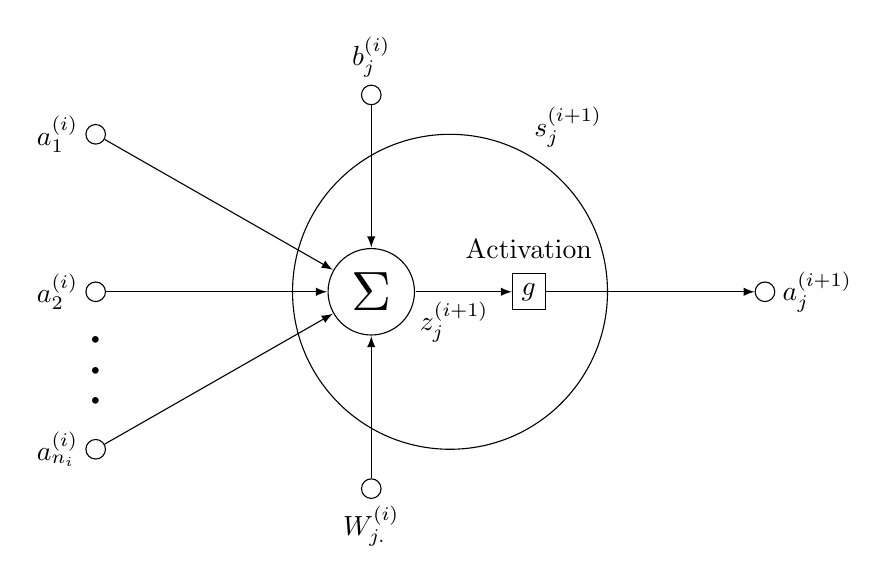
\begin{tikzpicture}[>=latex]
	\path
	(0,0)     		node[circle,draw,scale=2,inner sep=2pt] (S) {$\Sigma$}
	+(90:2.5) 		node[circle,draw,inner sep=2.5pt] 		(b) {}
	node[above=1mm] {$b_j^{(i)}$}
	+(-90:2.5) 		node[circle,draw,inner sep=2.5pt] 		(W) {}
	node[below=1mm] {$W_{j.}^{(i)}$}
	+(-3.5,2) 	 	node[circle,draw,inner sep=2.5pt] 		(a1) 	{}
	node[left=1mm]  {$a_1^{(i)}$}
	+(-3.5,0)    	node[circle,draw,inner sep=2.5pt]		(a2) 	{}
	node[left=1mm]  {$a_2^{(i)}$}
	+(-3.5,-2) 		node[circle,draw,inner sep=2.5pt]		(ai) 	{}
	node[left=1mm]  {$a_{n_i}^{(i)}$}
	(2,0)    		node[draw] 								(g) 	{$g$} node[above=3mm]{Activation}
	+(0:3)  		node[circle,draw,inner sep=2.5pt]  		(y1) 	{}
	node[right=1mm]  {$a_{j}^{(i+1)}$};
	\draw[->] (S)--(g) node[pos=.4,below]{$z_j^{(i+1)}$};
	\draw[->] (b)--(S);
	\draw[->] (W)--(S);
	\draw[->] (g)--(y1);
	\draw[->] (a1)--(S);
	\draw[->] (a2)--(S);
	\draw[->] (ai)--(S);
	%\draw[black] (1,0) circle(2) ;
	
	\node[draw,circle,minimum size=4cm,inner sep=0pt, label={[xshift=1.5cm, yshift=-0.3cm]$s_j^{(i+1)}$}] at (1,0) {};
	
	\path (a2) -- (ai) node [font=\Huge, midway, sloped] {$\dots$};
	\end{tikzpicture}
	
	\caption{Components of a single neuron.}
	\label{fig:neuron_notation}
\end{figure}


Having described the basic function of a single neuron in the previous section, the focus is now on how multiple neurons interact in order to form a neural network. Figure (\ref{fig:neuron_notation}) shows the same single neuron as figure (\ref{fig:simple_neuron}) but with a slightly adapted and extended notation. While in figure (\ref{fig:simple_neuron}) the weights $\omega_i$ are directly assigned to the individual inputs $x_i$, in figure (\ref{fig:neuron_notation}) these weights are represented by a weight vector $W_{j.}^{(i)}$. To be able to refer to a single neuron in a neural network with a large number of neurons, a single neuron is referred to in the form of $s_j^{(i)}$. Where $s$ stands for single neuron, $i$ for the layer in which the neuron is used and $j$ for a consecutive number over all neurons in this layer $i$. The notation of the inputs and the output of a neuron have also changed, so that the notation $a_j^{(i)}$ is now used in both cases. The $a$ refers to activation and the two indices $i$ and $j$ refer to the layer and respectively the neuron that generated the activation value. The value $a_1^{(i)}$ from figure (\ref{fig:neuron_notation}) therefore identifies both, the output of the first neuron in the i-th layer and the input for the j-th neuron in the i+1-th layer. Depending on which and how many layers, and how the individual neurons in the individual layers or between the individual layers are connected to each other, different types of neural networks result. So-called feedforward networks, for example, are characterized by the fact that neurons from one layer are only connected to neurons from the next higher layer. The information flow therefore takes place only in one direction, namely from the input side to the output side. On the other hand there are so-called recurrent nets where feedback between different layers is also allowed. There are three different categories of recurrent neural networks which can be distinguished depending on how they use their feedback signals \cite{rek_net}: 

\begin{itemize}
	\item Direct feedback: The own output of a neuron is used as an additional input for the neuron.
	\item Indirect feedback: The output of a neuron serves as an input to a neuron of a previous layer.
	\item Lateral feedback: The output of a neuron servers as an input to a neuron from the same layer.
\end{itemize}


\tikzset{%
	every neuron/.style={
		circle,
		draw,
		minimum size=1.25cm
	},
	neuron missing/.style={
		draw=none, 
		scale=4,
		text height=0.333cm,
		execute at begin node=\color{black}$\vdots$
	},
}

\begin{figure}
	\centering
	\begin{tikzpicture}[x=1.5cm, y=1.5cm, >=stealth]

	\foreach \m/\l [count=\y] in {1,2,3,missing,4}
	\node [every neuron/.try, neuron \m/.try] (input-\m) at (0,2.5-\y) {};
	
	\foreach \m [count=\y] in {1,missing,2}
	\node [every neuron/.try, neuron \m/.try ] (hidden1-\m) at (1.75,2-\y*1.25) {};
	
	\foreach \m [count=\y] in {1,missing,2}
	\node [every neuron/.try, neuron \m/.try ] (hidden2-\m) at (4.75,2-\y*1.25) {};
	
	\foreach \m [count=\y] in {1,missing,2}
	\node [every neuron/.try, neuron \m/.try ] (output-\m) at (6,1.5-\y) {};
	
	
	\node at (input-1) {$x_1$};
	\node at (input-2) {$x_2$};
	\node at (input-3) {$x_3$};
	\node at (input-4) {$x_{n_0}$};
	
	\node at (hidden1-1) {$s_1^{(1)}$};
	\node at (hidden1-2) {$s_{n_1}^{(1)}$};
	
	\node at (hidden2-1) {$s_1^{(N)}$};
	\node at (hidden2-2) {$s_{n_N}^{(N)}$};
	
	\node at (output-1) {$s_1^{(N+1)}$};
	\node at (output-2) {$s_{n_{N+1}}^{(N+1)}$};
	
	\draw [->] (output-1) -- ++(1,0) node [above, midway] {$\hat{y}_1$};
	\draw [->] (output-2) -- ++(1,0) node [above, midway] {$\hat{y}_{n_{N+1}}$};
	
	\foreach \i in {1,...,4}
	\foreach \j in {1,...,2}
	\draw [->] (input-\i) -- (hidden1-\j);
	
	\foreach \i in {1,...,2}
	\foreach \j in {1,...,2}
	\draw [->] (hidden1-\i) -- (hidden2-\j);
	
	\foreach \i in {1,...,2}
	\foreach \j in {1,...,2}
	\draw [->] (hidden2-\i) -- (output-\j);
	
	\node [align=center, above] at (0,2) {Input\\layer};
	\node [align=center, above] at (1.75,2) {Hidden \\layer 1};
	\node [align=center, above] at (4.75,2) {Hidden \\layer N};
	\node [align=center, above] at (6,2) {Output \\layer};
	
	\node[fill=white,scale=4,inner xsep=0pt,inner ysep=5mm] at ($(hidden1-1)!.5!(hidden2-2)$) {$\dots$};

	\end{tikzpicture}
	\caption{Illustration of fully connected feedforward neural network with $N$ hidden layers.}
	\label{fig:feedforward_network}
\end{figure}	

Since the possibilities of how the different neurons are connected in a neural network are almost unlimited, the following section describes one of the most common forms \cite{kriesel}. It is a fully connected feedforward network as shown in figure (\ref{fig:feedforward_network}). The most important properties of such a network are:

\begin{itemize}
	\item Fully connected: All outputs from the neurons of layer $i$ serve as inputs for all neurons in layer $i+1$.
	\item Feedforward: The information flows only from one layer to the next higher layer. 
\end{itemize}

For the calculation and analysis of such a neural network the following notation, which is taken from \cite{Mar_Pri}, is used in accordance with figure (\ref{fig:neuron_notation}) and (\ref{fig:feedforward_network}). Let

\begin{itemize}
	\item $N \in \N$ be the number of hidden layers in the neural network.
	
	\item $N + 2$ be the total number of layers in the network since the hidden layers are wrapped between an input and an output layer. 
	
	\item $n_i \in \N, i \in \{0, 1, ..., N+1\}$, be the number of neurons in the $i$-th layer.
	
	\item $s_j^{(i)}$ denote the $j$-th neuron of the $i$-th layer. 
	
	\item $a^{(i)} \in \R^{n_i}$, $a^{(i)} = (a_1^{(i)}, a_2^{(i)}, ..., a_{n_i}^{(i)})^\top$ be the vector of activation values produced by the neurons of the $i$-th layer.
	
	\item $b^{(i)} \in \R^{n_{i+1}}$, $b^{(i)} = (b_1^{(i)}, b_2^{(i)}, ..., b_{n_{i+1}}^{(i)})^\top$ be the bias vector for the linear transformation performed in all neurons of layer $i+1$.

	\item $W_{j.}^{(i)} \in \R^{1 \times n_i}$, $W_{j.}^{(i)} = (W_{j1}^{(i)}, W_{j2}^{(i)}, ..., W_{jn_i}^{(i)})$ be the weight vector for the linear transformation performed in the $j$-th neuron of the $i+1$-th layer. Combining all weights used in the $i+1$-th layer into a matrix $W^{(i)} \in \R^{n_{i+1} \times n_i}$ results in:	
		\begin{align*}
		W^{(i)} = 
		\begin{pmatrix}
		W_{11}^{(i)}		& W_{12}^{(i)}		 	& \cdots 	& W_{1n_i}^{(i)}	 \\
		W_{21}^{(i)}		& W_{22}^{(i)}			& \cdots 	& W_{2n_i}^{(i)} 	\\
		\vdots 				& \vdots 		 	 	&			& \vdots 		\\
		W_{n_{i+1}1}^{(i)}	& W_{n_{i+1}2}^{(i)}	& \cdots 	& W_{n_{i+1}n_i}^{(i)} 
		\end{pmatrix}
		= 
		\begin{pmatrix}
		W_{1.}^{(i)}\\
		W_{2.}^{(i)}\\
		\vdots \\
		W_{n_{i+1}.}^{(i)} 
		\end{pmatrix},
		\end{align*}		
	with $W_{j.}^{(i)}$ being the $j$-th row of $W^{(i)}$.
	
	\item $z^{(i)} \in \R^{n_i}$, $z^{(i)} = (z_1^{(i)}, z_2^{(i)}, ..., z_{n_i}^{(i)})^\top$ be the result vector after the linear transformation performed in all neurons of layer $i$.
	
	\item $g: \R \mapsto \R$ be any activation function which is applied to the result of the linear transformation. 
	
	\item $x \in \R^{n_0}$, $x = (x_1, x_2, ..., x_{n_0})^\top$ be a vector of input data to train the model. 
	
	\item $y \in \R^{n_{N+1}}$, $y = (y_1, y_2, ..., y_{n_{N+1}})^\top$ be a vector of output data to train the model. 
	
	\item $\hat{y} \in \R^{n_{N+1}}$, $\hat{y} = (\hat{y}_1, \hat{y}_2, ..., \hat{y}_{n_{N+1}})^\top$ be a vector of estimated output values obtained from the neural network by sending an input vector $x$ through the network. 
\end{itemize}

\begin{remark}
	Since the input layer has $n_0$ neurons, the input vector $x$ must be an element of $\R^{n_0}$. Similarly, the estimated output $\hat{y}$ of the neural network is a vector which is an element of $\R^{n_{N+1}}$.
\end{remark}

\begin{remark}
	Since $a^{(i)}$ denotes the values that are transferred between neurons, it is both the output values of the neurons from layer $i$ and the input values of the neurons from layer $i+1$. 
\end{remark}

\begin{remark}
	The input values $x$ for the neuronal network correspond to the first activation values $a^{(0)}$, e.g. $x = a^{(0)}$. Similarly, the estimated output $\hat{y}$ of the neural network corresponds to the last activation values $a^{(N+1)}$, e.g. $\hat{y} = a^{(N+1)}$.
\end{remark}

\begin{remark}
	For the training of a neural network many different sets of input and associated output vectors are needed.	If a specific set of input or output data is to be referenced, this is done by adding a superscript, e.g. $x^{(k)}$ and $y^{(k)}$. The corresponding estimated values are also referred to as $\hat{y}^{(k)}$. 
\end{remark}
\begin{remark}
	The weight defined as $W_{jk}^{(i)}$ connects the activation value from the $k$-th neuron in layer $i$ with the $j$-th neuron from layer $i + 1$.
\end{remark}

After a notation for the analysis of the neural network has been defined, the next section is devoted to the question of how data can flow through a network and how the network can learn. 

\section{Train a model}

Figure (\ref{fig:simple_neuron}) together with formula (\ref{eq:simple_neuron}) already illustrated in the previous section how a single neuron is constructed and how it processes the inputs. Since the notation has been generalized in the previous section also formula (\ref{eq:simple_neuron}) could be generalized. 

\begin{remark}
	Let $a^{(i)} \in \R^{n_i}$ be the activation values from layer $i$, $b_j^{(i)} \in \R$ the bias term for the $j$-th neuron in layer $i+1$, $W_{j.}^{(i)}$ the weights and $g: \R \mapsto \R$ any activation function. Then the linear transformation performed by the $j$-th neuron of layer $i+1$ called $s_j^{(i+1)}$ is given by:
	\begin{equation}
		z_j^{(i+1)} = \sum_{k=1}^{n_i} W_{jk}^{(i)} a_k^{(i)} + b_j^{(i)}
	\end{equation}
	Using vector notation gives:
	\begin{equation}
		z_j^{(i+1)} = W_{j.}^{(i)} a^{(i)} + b_j^{(i)}
	\end{equation}	
\end{remark}

\begin{remark}
	Based on the previous remark, the activation value $a_j^{(i+1)}$ generated by neuron $s_j^{(i+1)}$ is given by: 
	\begin{equation}
		a_j^{(i+1)} = g(z_j^{(i+1)}) = g \bigg( \sum_{k=1}^{n_i} W_{jk}^{(i)} a_k^{(i)} + b_j^{(i)} \bigg) \\
	\end{equation}
	Using vector notation gives:
	\begin{equation}
		a_j^{(i+1)} = g(z_j^{(i+1)}) = g( W_{j.}^{(i)} a^{(i)} + b_j^{(i)} )
	\end{equation}	
\end{remark}

Performing these transformations for all neurons from layer $i+1$ gives a system of $n_{i+1}$ equations:
\begin{align*}
	a_1^{(i+1)} &= g( W_{1.}^{(i)} a^{(i)} + b_1^{(i)} ) 	\\
	a_2^{(i+1)} &= g( W_{1.}^{(i)} a^{(i)} + b_1^{(i)} ) 	\\
				&\vdots										\\	
	a_{n_{i+1}}^{(i+1)} &= g( W_{1.}^{(i)} a^{(i)} + b_1^{(i)} )
\end{align*}
Since the activation function is only defined for scalar values, a small extension must be made.

\begin{remark}
	Let $g: \R \mapsto \R$ be an activation function which operates on scalars only. In case that an vector is supplied the scalar activation function $g$ is applied element by element. 
\end{remark}

With the help of the previous remark it is now possible to represent the flow of information through the network in vector notation.
\begin{equation}
\begin{aligned}
	a^{(0)} 	&= x								\\
	z^{(i)} 	&= W^{(i-1)} a^{(i-1)} + b^{(i-1)} 	\\
	a^{(i)}		&= f(z^{(i)}) 						\\
	a^{(N+1)} 	&= \hat{y}
\end{aligned}
\end{equation}

This step, where the neural network takes an input vector and transforms it to a prediction is the first step to train the network and is called forward propagation \cite{Propagation}. The process shown in the figure (\ref{fig:NN_overview}) illustrates that after the generation of the predictions $\hat{y}$ the deviation between these and the real outputs $y$ must be measured. A way of measuring the deviation between actual and estimated values is the $L^2$ norm.

\begin{definition}
	Let $x^{(i)}$ and $y^{(i)}$ be the vector of the input and the corresponding output values, respectively. Let $W$ be the matrices of weights and $b$ the vectors of biases used in the entire network for a single forward propagation. If $\hat{y}_{W,b,x^{(i)}}^{(i)}$ denotes the estimated outputs from the network then the loss score is given by:	
	\begin{equation}\label{eq:single_loss}
		L(b, W, x^{(i)}, y^{(i)}) := \frac{1}{2} \norm{\hat{y}_{W,b,x^{(i)}}^{(i)} - y^{(i)}}^2_2
	\end{equation}
\end{definition}

By using the notation given in equation (\ref{eq:single_loss}) it is explicitly stated, that the loss of a single forward pass depends on the four parameters $b, W, x^{(i)}$ and $y^{(i)}$. In order to increase the readability in the following paragraphs from now on it is not longer explicitly stated that the estimated output depends on the three parameters $W$, $b$ and $x^{(i)}$, e.g. $\hat{y}_{W,b,x^{(i)}}^{(i)} = \hat{y}$. Since in most cases not only a single pair of input and output data is used for the calculation of the loss function but several, the loss must also be defined for a sample of multiple input and output vectors. In the field of machine learning such a sample of multiple input and output vectors is called a batch. The batch size is one of the so-called hyperparameters of a neural network and specifies how many samples must be sent through the network before the model parameters are updated.

\begin{definition}\label{def:batch_loss}
	Let $\{(x^{(1)}, y^{(1)}), (x^{(2)}, y^{(2)}), ..., (x^{(m)}, y^{(m)})\}$ be a sample of $m$ input and the corresponding output vectors, e.g. the batch size is $m$. Then the loss is given by:	
	\begin{equation}\label{eq:multiple_loss}
	\begin{aligned}
	L(b, W) &= \frac{1}{m} \sum_i^m \frac{1}{2} \norm{\hat{y}^{(i)} - y^{(i)}}^2_2 \\
			&= \frac{1}{m} \sum_i^m L(b, W, x^{(i)}, y^{(i)})
	\end{aligned}
	\end{equation}
\end{definition}

\begin{remark}
	In order to reduce the complexity of the model by using smaller weights and to reduce overfitting to some extend, a regularization term can be used in equation (\ref{eq:multiple_loss}).
	\begin{equation}\label{eq:multiple_loss_regularization}
	\begin{aligned}
	L(b, W) &= \frac{1}{m} \sum_i^m \frac{1}{2} \norm{\hat{y}^{(i)} - y^{(i)}}^2_2 + \frac{\lambda}{2} \sum_{i=0}^{N} \norm{W^{(i)}}_F^2\\
	&= \frac{1}{m} \sum_i^m L(b, W, x^{(i)}, y^{(i)}) + \lambda R(W)
	\end{aligned}
	\end{equation}
\end{remark}

If a regularization term is used in a neural network, the choice of the regularization parameter $\lambda$ plays an important role. When the regularization term $\lambda$ is too high the weight matrices $W$ are close to zero and this can lead to simple networks and underfitting. However, if the parameter is set too low and therefore higher weights of the matrices are not penalized enough, regularization has no effect at all.

Once a loss function is defined, the information of the loss score can be used to take the next step as shown in the figure (\ref{fig:NN_overview}). The job of the optimizer is to evaluate how the weights of $W$ and $b$ have to be adjusted so that the loss score becomes smaller in the next forward pass. A reduction of the loss score indicates that the deviation between predicted output values and actual outputs is reduced. This iterative improvement of the loss score based on the insights given by the optimizer is the so called learning procedure of a neural network. The task of minimizing $L(b, W)$ with respect to the weights $b$ and $W$ can be solved by using the gradient descent method which is an  first-order iterative optimization algorithm for finding the local minimum of a function \cite{gradient_desc}. Within each step of the iterative procedure the weights of the network are then gradually adjusted with a constant learning rate of $\alpha$. 

\begin{remark}
	Let $W^{(i)}$ and $b^{(i)}$, $i = 0, 1, ..., N$ be the weights used in the $i+1$-th layer and $\alpha \in  \R_+$ the user defined learning rate. Then the weights are updated in every optimization step such that:
	\begin{align}
	b_j^{(i)} 		&= b_j^{(i)} - \alpha \frac{\partial}{\partial b_j^{(i)}} L(b, W)\\
	W_{jk}^{(i)} 	&= W_{jk}^{(i)} - \alpha \frac{\partial}{\partial W_{jk}^{(i)}} L(b, W)
	\end{align}	
\end{remark}

By using definition \ref{def:batch_loss} the update process is given as:



The only unknowns in the formulas a and b are now the partial derivatives for a given learning rate alpha.
backpropagation strictly refers only to the algorithm for computing the gradient,

